\documentclass[tikz]{standalone}
\usepackage{pgfplots}
\pgfplotsset{compat=1.15}
\usepackage{mathrsfs}
\usetikzlibrary{arrows,calc}
\usepackage{tkz-euclide}

\pagestyle{empty}

\definecolor{AngleClr}{rgb}{0,0.39215686274509803,0}
\definecolor{ShapeClr}{rgb}{0.6,0.2,0}

\begin{document}

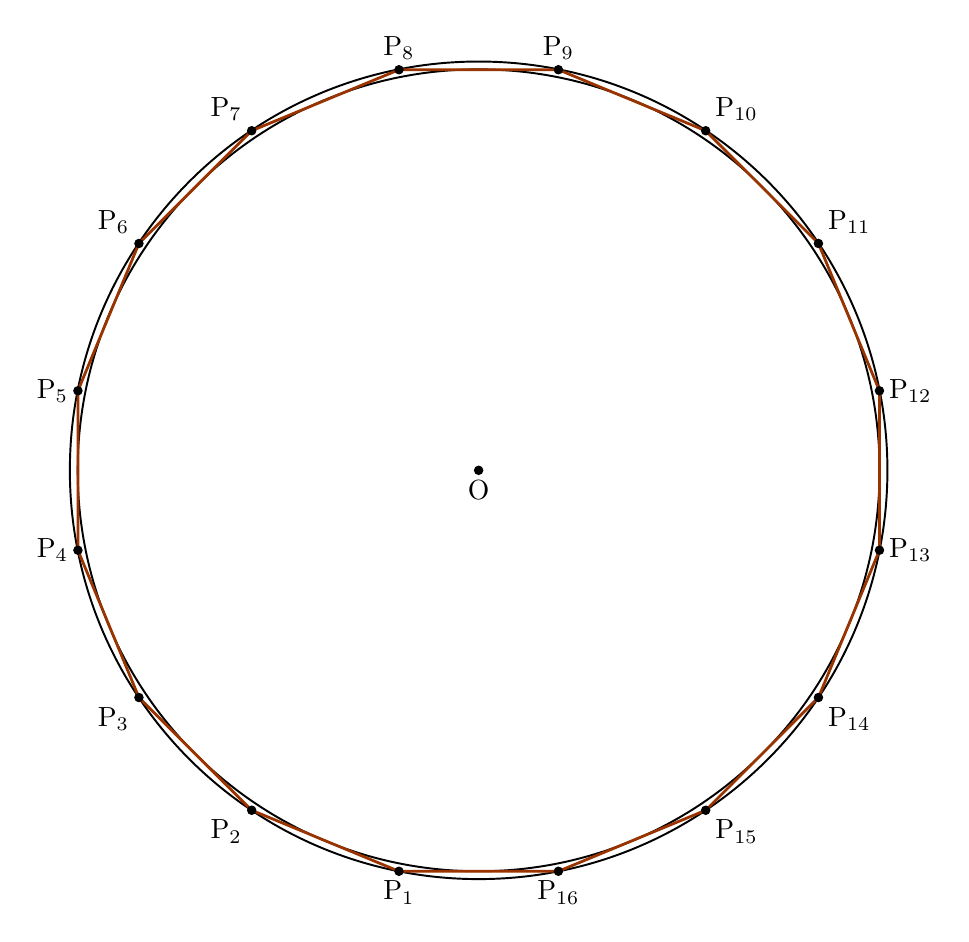
\begin{tikzpicture}[scale=.75]
\tkzSetUpLine[line width=1pt,color=black]
\tkzSetUpPoint[fill=black]

\tkzDefPoints{0/0/P0,2.7/0/P1}

\tkzDefRegPolygon[side,sides=16](P0,P1)

\tkzDefMidPoint(P1,P2) \tkzGetPoint{M1}
\tkzDefMidPoint(P2,P3) \tkzGetPoint{M2}
\tkzDefMidPoint(P3,P4) \tkzGetPoint{M3}
\tkzDefMidPoint(P4,P5) \tkzGetPoint{M4}
\tkzDefMidPoint(P5,P6) \tkzGetPoint{M5}
\tkzDefMidPoint(P6,P7) \tkzGetPoint{M6}
\tkzDefMidPoint(P7,P8) \tkzGetPoint{M7}
\tkzDefMidPoint(P8,P9) \tkzGetPoint{M8}
\tkzDefMidPoint(P9,P10) \tkzGetPoint{M9}
\tkzDefMidPoint(P10,P11) \tkzGetPoint{M10}
\tkzDefMidPoint(P11,P12) \tkzGetPoint{M11}
\tkzDefMidPoint(P12,P13) \tkzGetPoint{M12}
\tkzDefMidPoint(P13,P14) \tkzGetPoint{M13}
\tkzDefMidPoint(P14,P15) \tkzGetPoint{M14}
\tkzDefMidPoint(P15,P16) \tkzGetPoint{M15}
\tkzDefMidPoint(P16,P1) \tkzGetPoint{M16}


\tkzFillPolygon[fill=white](P1,P2,P3,P4,P5,P6,P7,P8,P9,P10,P11,P12,P13,P14,P15,P16)

\tkzDefCircle[circum](P1,P2,P3) \tkzGetPoint{O}
\tkzDrawCircle[line width=0.7pt,black](O,P1)
\tkzDrawCircle[line width=0.7pt,black](O,M1)


\tkzDrawPolygon[color=ShapeClr](P1,P2,P3,P4,P5,P6,P7,P8,P9,P10,P11,P12,P13,P14,P15,P16)
\tkzDrawPoints[size=3](O,P1,P2,P3,P4,P5,P6,P7,P8,P9,P10,P11,P12,P13,P14,P15,P16)
\tkzLabelPoint[below](P1){$\rm P_1$}
\tkzLabelPoint[below](P2){$\rm P_{16}$}
\tkzLabelPoint[below right](P3){$\rm P_{15}$}
\tkzLabelPoint[below right](P4){$\rm P_{14}$}
\tkzLabelPoint[right](P5){$\rm P_{13}$}
\tkzLabelPoint[right](P6){$\rm P_{12}$}
\tkzLabelPoint[above right](P7){$\rm P_{11}$}
\tkzLabelPoint[above right](P8){$\rm \rm P_{10}$}
\tkzLabelPoint[above](P9){$\rm \rm P_9$}
\tkzLabelPoint[above](P10){$\rm P_8$}
\tkzLabelPoint[above left](P11){$\rm P_7$}
\tkzLabelPoint[above left](P12){$\rm P_6$}
\tkzLabelPoint[left](P13){$\rm P_5$}
\tkzLabelPoint[left](P14){$\rm P_4$}
\tkzLabelPoint[below left](P15){$\rm P_3$}
\tkzLabelPoint[below left](P16){$\rm P_2$}

\tkzLabelPoint[below](O){$\rm O$}

\end{tikzpicture}

\end{document}
